\section{Diseño Estructural}\label{sec:dis_estructural}
Este trabajo de tesis plantea una arquitectura a nivel de sistema.
Esta arquitectura se encuentra basada en la red CAN debido a
un interés especial de INVAP. Además se sigue una filosofía de red
distribuída por las razones estudiadas en la sección
\ref{seccion:TopologiaEstudio}. Esto le da la característica de innovador
a este proyecto, ya que no se encontró en estado de la cuestión
la utilización de esta filosofía en el desarrollo de vehículos
espaciales, mucho menos en Argentina, que se sigue una filosofía
más tradicional y conservadora a la hora de desarrollar satélites. 

La arquitectura propuesta, como se mencionó anteriormente tiene como
base el bus CAN. A la red se pueden conectar un número N de
nodos ( N < 128 ), siendo estos componentes COTS de baja confiabilidad. 
Esta arquitectura trabaja en las capas superiores 
de los protocolos de comunicación, por lo tanto, en esta instancia 
de trabajo, el nodo se conecta a la red mediante un microcontrolador 
CAN, el cual a su vez está compuesto por el CAN tranceiver.

La red a bajo nivel, es decir desde el cable CAN, el CAN Tranceiver y 
el microcontrolador CAN, deben trabajar bajo las normas preestablecidas
por algún protocolo existente, que cuya selección de este, cae bajo la 
responsabilidad del diseñador y/o ingeniero de sistemas que vaya 
a implementar la arquitectura. Para esta arquitectura se aconseja el uso
del protocolo CANOpen \citep{can-ciaWEB}. Esto se puede observar en la
 Figura \ref{fig:DiagramaEstructuraCompleta} que el Node (nodo de la red)
tiene como \textit{inout flowport} el microcontrolador CAN  y el
CAN Tranceiver. El CAN Tranceiver simplemente emite y recibe señales eléctricas. Las 
especificaciones (por ejemplo resitencias y voltaje, que son mostrados en el diagrama
solo con propósito) se pueden encontrar en los estándares \citep{can-ciaWEB}.

\begin{figure}[h!]
 \centering
 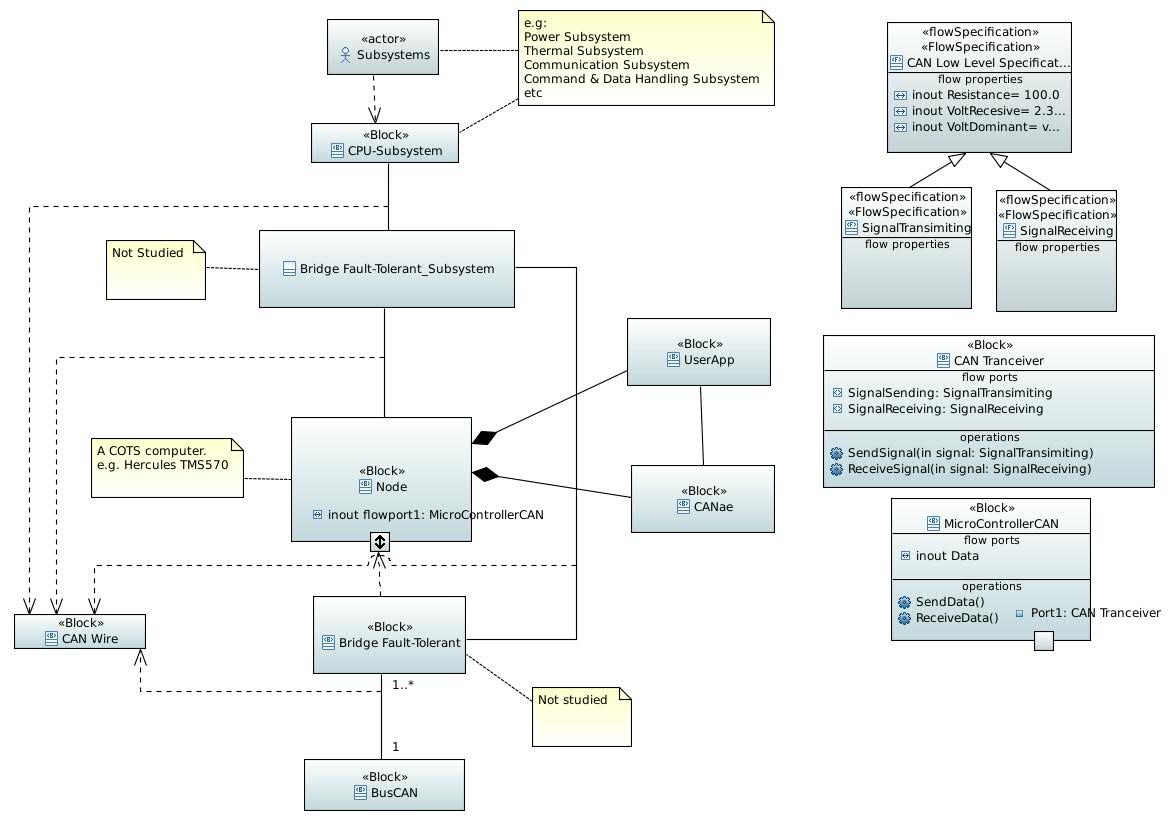
\includegraphics[scale=0.4]{images/Capitulo5/ArqCompletaBlockDiagram.JPG}
  \caption{Diagrama de bloques de la arquitectura completa}
\label{fig:DiagramaEstructuraCompleta}
\end{figure} 

Dentro de cada nodo se encuentra la aplicación de usuario que será de 
responsabilidad del desarrollador implementar esta aplicación haciendo uso
del protocolo CANae desarrollado en este trabajo.

Para agregar tolerancia a fallas a la arquitectura se plantea la necesidad de 
llevar a cabo un Bridge tolerante a fallas. Este Bridge permite que la comunicación de la red
con los subsistemas no se vean afectadas ante la falla de un nodo. La utilización
de esta técnica se explica en la siguiente sección.

De esa manera queda definida la estructura a nivel de bloques de la arquitectura
planteada. 

\subsection{Bridge tolerante a fallas}\label{subsec:bridge}
En esta sección se explica la necesidad de la utilización de un Bridge 
Tolerante a Fallas. No se pretende llevar a cabo una especificación técnica
del Bridge, ya que escapan a los propósitos de este trabajo de tesis. 
En primer lugar, como la arquitecutra persigue la filosofía de red distribuida, 
y la posibilidad de distribuir las tareas entre todos los nodos, surge la 
dificultad de que muchas veces no existe compatibilidad entre las computadoras 
de los diferentes subsistemas. Es decir, una computadora del subsistema 
de control térmico, por ejemplo, no puede prender y/o pagar componentes del 
subsistema de propulsión. Tal como se muestra en la Figura \ref{fig:Bridge1} la 
ejecución de tareas de un subsistema en otro está prohíbido. 

\begin{figure}[h!]
 \centering
 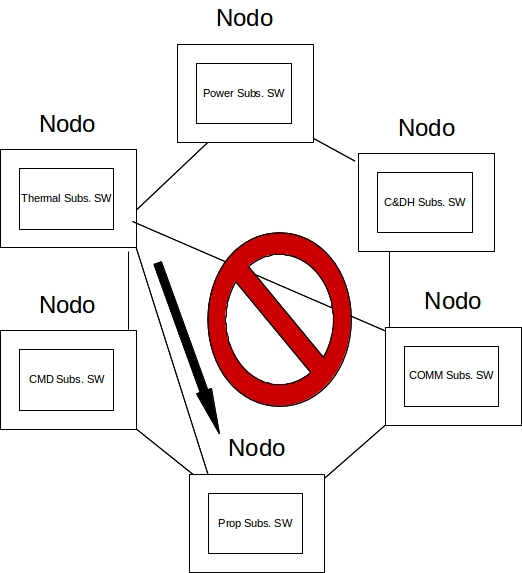
\includegraphics[scale=0.6]{images/Capitulo5/Bridge1.jpg}
  \caption{Posibilidad de interconexión de nodos.}
\label{fig:Bridge1}
\end{figure} 

Esto lleva a una segunda propuesta en la cual el nodo conectado 
a la red distribuida, debe estar separado de la computadora que 
se comunican directamente con los componentes del subsistema. Con esto
surge una segunda propuesta de desarrollo de la estructura de arquitectura.
En esta, el subsistema se encuentra separado del nodo, con su propia CPU, y se conecta
a la red mediante el nodo. Suponiendo que un nodo falle,
 debido a su baja confiabilidad (es un componente COTS), ese subsistema queda totalmente
aislado de la red. En la Figura \ref{fig:Bridge2} se observa que, cuando falla el Nodo
del \textit{Subsistema 1} cualquier mensaje que envíe el \textit{Subsistema 2} al primero, 
nunca se entregará. Esto provoca que la confiabilidad del sistema completo, disminuya 
linealmente con la confiabilidad del componente COTS. 

\begin{figure}[h!]
 \centering
 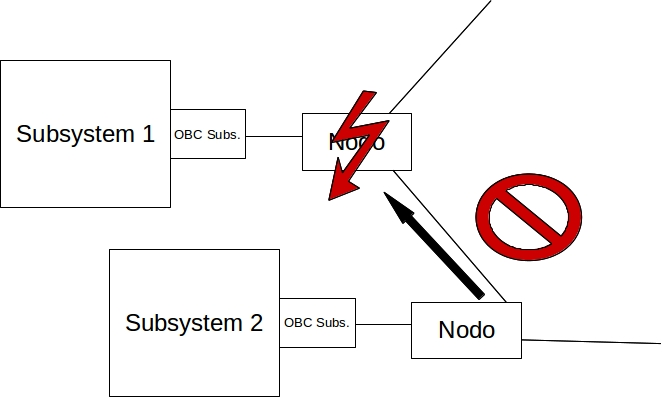
\includegraphics[scale=0.6]{images/Capitulo5/Bridge2.jpg}
  \caption{Posibilidad de interconexión de nodos.}
\label{fig:Bridge2}
\end{figure} 

La tercera opción y la ideal es la existencia de un Bridge, que se lo llama: 
\textit{Bridge Tolerantes a Fallas}. Esto crea un puente entre la red y la computadora
del subsistema permitiendo aumentar la tolerancia a fallas de la arquitectura. En 
caso de fallas en el nodo, el Bridge se activa ignorando al \textit{nodo fallado} y 
conectando a la computadora del subsistema directamente en la red.  Esto se puede observar
en la Figura \ref{fig:conn_prop}, siendo el Bridge el cuadrado negro.

\begin{figure}[h!]
 \centering
 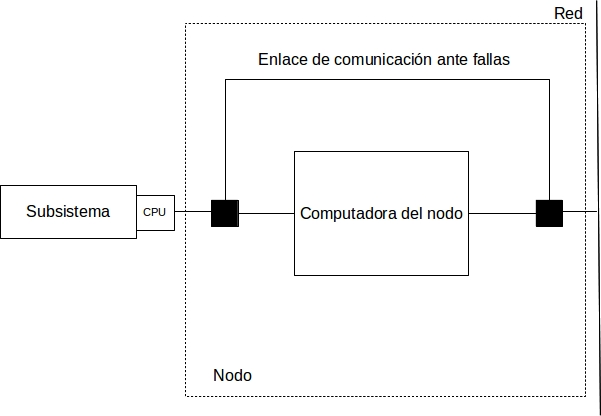
\includegraphics[scale=0.6]{images/Capitulo4/com_nodo.jpg}
 \caption{Conexión entre la red y el subsistema}
\label{fig:conn_prop}
\end{figure}

Los detalles técnicos, electrónicos y de implementación no se desarrollan en
este trabajo de tesis. 

Como puede observarse en al Figura \ref{fig:DiagramaEstructuraCompleta} el
protocolo CANae se encuentra dentro del nodo. El desarrollador se debe encargar
de implementar los protocolos, como un stack de servicios más del 
sistema operativo (o sistema embebido) que se encuentre en el nodo.

\subsection{Bloques Internos}
En esta sección se muestra el diagrama de bloques internos que conforman el
nodo que es aquel que implementa el protocolo de comunicación CANae. Como
puede observarse en la Figura \ref{fig:BloquesInternosArq} el nodo, representa
la parte más compleja de la red. En este dispositivo se encuentra toda la
complejidad de la arquitectura, y es el encargado tanto de llevar a cabo
las tareas, como así también comunicarse con los demás nodos, a través del
protocolo CANae y coordinar las tareas a desarrollarse. Además,
debe notarse que estos nodos se suponen que son componentes de estantería
o componentes \ac{COTS} los cuales tiene una muy baja confiabilidad, pero con 
un alta perfomance. Por lo tanto, es de esperarse que el software de los
nodos esté basado o dearrollado sobre un Sistema Operativo de Tiempo
Real (RTOS) y estos deben aplicar técnicas de tolerancia a fallas que
escapan de los alcances de este trabajo de tesis. Todos los bloques
internos que se observa en la Figura \ref{fig:BloquesInternosArq} deben
desarrollarse como módulos pertenecientes al stack del servicio del
sistema operativo, o bien, módulos de servicio del sistema embebido de
los nodos.

Como se estudió en el marco teórico (Véase sección \ref{seccion:ProtocoloCAN})
el estándar del protocolo CAN \citep{can-ciaWEB} trabaja en las capas
inferiores del modelo de OSI. Cada Nodo que se deba conectar a una red basada
en CAN debe, en primer lugar, contar con un CAN Tranceiver y un
Microcontrolador CAN, estos son modelados en el diagrama de bloques
internos como Ports. CANae (Véase apéndice \ref{Appendix:A}) por su parte,
trabaja en la capa de aplicación del modelo de OSI. Esta es modelada como
una Parte (Part) del Nodo. Como se puede observar en el modelo
\ref{BloquesInternosArq}, CANae es la capa de comunicación de la red
que se comunica directamente (como es de esperarse) con la aplicación
del usuario. 

\begin{figure}[h!]
 \centering
 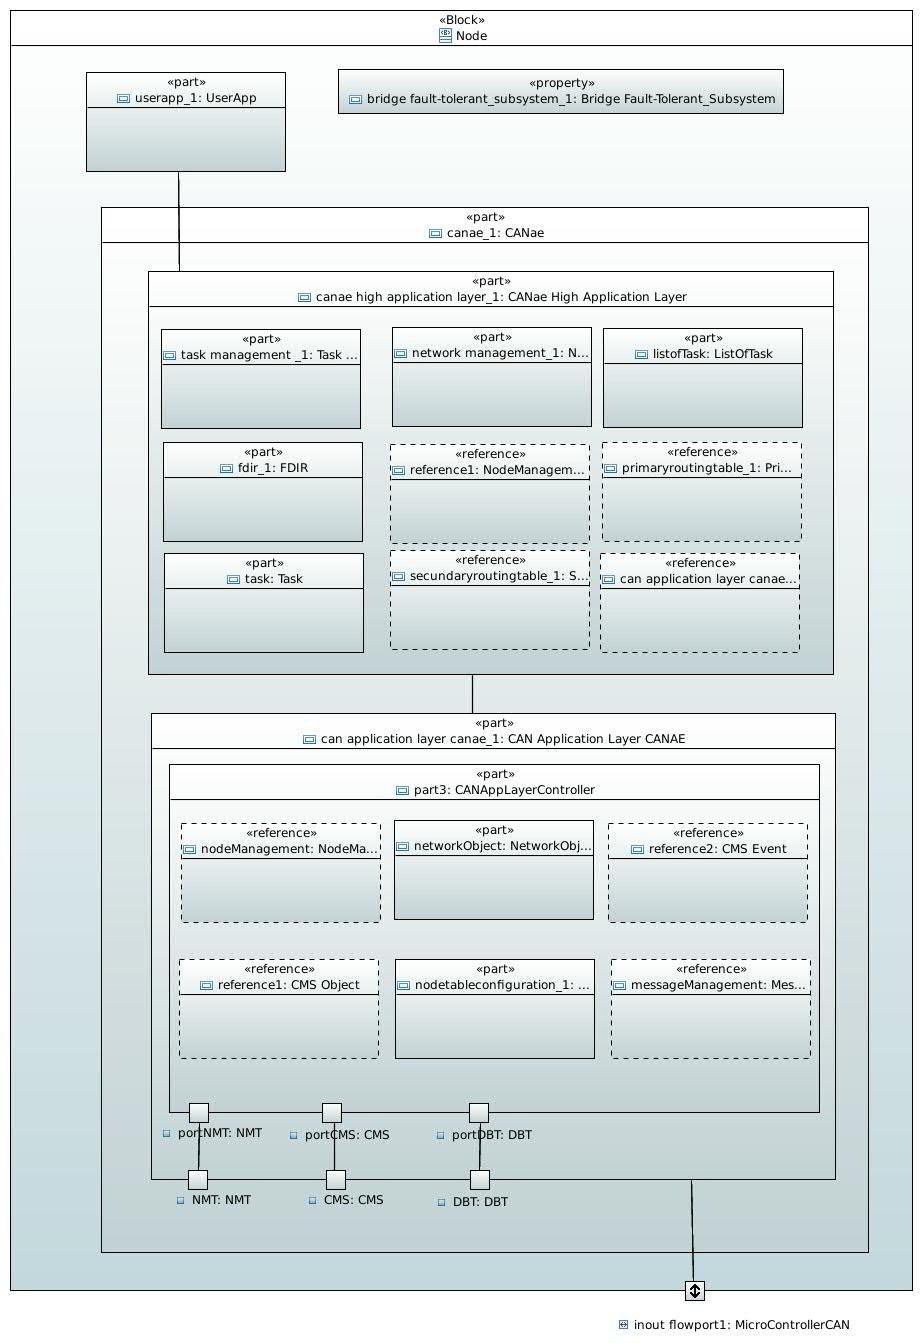
\includegraphics[scale=0.5]{images/Capitulo5/NodeInternalDiagram.JPG}
 \caption{Diagrama de bloques interno del nodo.}
\label{fig:BloquesInternosArq}
\end{figure}

\subsection{Nodo Monitor}
En la versión actual del protocolo CANae (0.1 Alpha) se preve la existencia de un
nodo monitor. El objetivo principal de este nodo es lograr la coordinación 
de todos los nodos en las fases de iniciación del protocolo. Una vez que la red
CANae ya fue creada, el nodo monitor  puede ser retirado.
